\chapter{卖出跨式价差\label{CH20}}
卖出跨式价差涉及\textbf{卖出一手看跌期权和一手条款相同的看涨期权}。同任何种类的期权卖出一样,卖出跨式价差可以是备兑的或未备兑的。这两种策略都使用得相当普遍。
\section{卖出备兑跨式价差}
在这种策略里,交易者在持有标的股票的同时卖出一手这个股票上的跨式价差。对那些已经涉足卖出备兑看涨期权的投资者,这种策略特别有吸引力。在现实中,这个头寸并不是完全备兑的,只有卖出的看涨期权部分才为持有的股票所保护。卖出的看跌期权是未备兑的。不过,“备兑跨式价差”的名字一般用在这类头寸上,以便将它同卖出未备兑跨式价差进行区分。
\begin{tcolorbox}
    XYZ 的价格为 51,XYZ 1 月 50 看涨期权的售价为 5 点,XYZ 1 月 50 看跌期权的售价为 4 点。一手卖出备兑跨式价差可以通过在买入 100 股标的股票的同时卖出 1 手看跌期权和 1 手看涨期权而建立起来。这个头寸同一手卖出备兑看涨期权头寸之间的相似性是相当明显的。卖出备兑跨式价差实际上是一手卖出备兑(买入 100 股 XYZ 加上卖出 1 手看涨期权)和一手卖出裸看跌期权组合而成的。
\end{tcolorbox}

\begin{figure}
    \begin{center}
        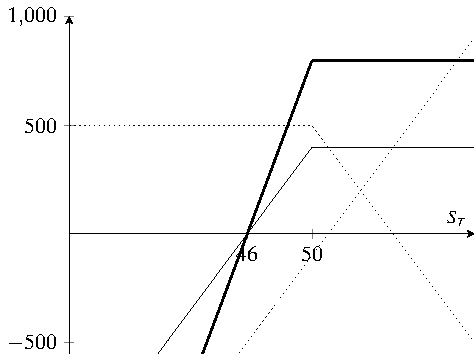
\includegraphics[width=0.8\textwidth]{IMG/fig20-1.pdf}
        \caption{卖出备兑跨式价差}
    \end{center}
\end{figure}

应当记得,卖出裸看跌期权与卖出备兑看涨期权相等。因此,一手卖出备兑跨式价差可以认为是同一个 200 股的卖出备兑看涨期权相等,或者是同卖出两手裸看跌期权相等。

事实上,备兑跨式价差的最大潜在盈利可以通过下面的公式很快计算出来:
\begin{equation}
    \begin{aligned}
        \text{最大盈利}   & =\text{跨式价差权利金}+\text{行权价}-\text{最初股票价格}         \\
        \text{盈亏平衡价格} & =\frac{\text{股票价格}+\text{行权价}-\text{跨式价差权利金}}{2} \\
    \end{aligned}
\end{equation}

备兑看涨期权卖出者可以变成备兑跨式价差卖出者,这样做的吸引人之处在于他可以不必显著地改变他的卖出备兑看涨期权头寸的系数,就可以增加他的收益。如果交易者决定通过用 51 买入 XYZ 和用 5 点卖出 1 月 50 看涨期权来建立一手卖出备兑,那么,他就有了一个最大潜在盈利在 50 之上,盈亏平衡点在 46 的头寸。如果在他的备兑看涨期权的头寸里加进那手裸看跌期权,他没有改变头寸的价格系数;他仍然可以在股票价格高于 50 时得到最大盈利,盈亏平衡点仍然是 46。因此,在变成备兑跨式价差卖出者的时候,他不必改变他对这个标的股票的看法。

由于加进了这手裸看跌期权,投资增加了,在到期时,在股票价格到50之上的潜在盈利金额增加了,在股票价格到 46 之下的潜在亏损金额也增加了。备兑跨式价差卖出者在下行方向亏损的速度要高出一倍,因为这个头寸同一个 200 股的卖出备兑相等。因为裸看跌期权的手续费比卖出备兑看涨期权的手续费要低,备兑看涨期权卖出者在他的头寸中加进一手裸看跌期权时,一般而言可以在某种程度上增加他的收益。

实施后续行动的方法同卖出备兑看涨期权基本相同。一般在备兑的情况中需要将看涨期权挪仓的时候,交易者现在都可以将整个跨式价差挪仓(向下挪仓以寻求保护,向上挪仓以增加盈利,如果跨式价差中的时间价值消失,那么就向前挪仓)。上下挪仓也许会涉及支出,除非是挪到更远的到期日。
\section{卖出无备兑跨式价差}
在一个卖出无备兑跨式价差中,交易者在没有持有标的股票的情况下卖出跨式价差。从广义上说,这是一个潜在盈利有限但潜在风险巨大的中性策略。不过,获得盈利的概率相当大,而且可以采用一定的方法来减小这个策略的风险。

因为交易者在这个策略中是在卖出一手看跌期权和一手看涨期权,他一开始得到大量的时间价值。如果标的股票价格在到期日相对没有变化,跨式价差的卖出者就可以就它的内在价值而将这个跨式价差买回来。这样做一般会带来一笔盈利。

\begin{tcolorbox}
    有下列价格存在:
    \begin{itemize}
        \item XYZ 普通股股票:45
        \item XYZ 1 月 45 看涨期权:4
        \item XYZ 1 月 45 看跌期权:3
    \end{itemize}
    一个跨式价差可以卖出 7 点。如果股票价格在到期日高于 38 或低于 52,这个跨式价差的卖出者就会盈利。因为在这个情况里,用少于 7 点就可以把实值期权买回来,而虚值期权则会无价值到期。
\end{tcolorbox}

\begin{figure}
    \begin{center}
        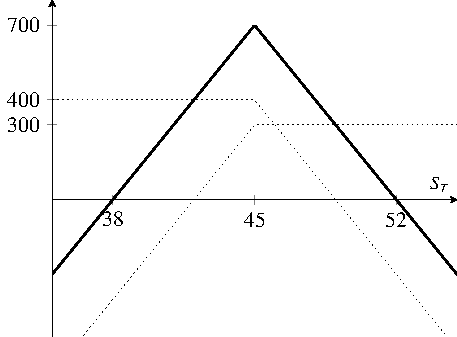
\includegraphics[width=0.8\textwidth]{IMG/fig20-2.pdf}
        \caption{卖出裸跨式价差}
    \end{center}
\end{figure}

\section{卖出跨式价差的选择}
理想情况下,交易者想要从卖出跨式价差中得到一笔权利金,它可以产生一个盈利范围,其宽度同标的股票的波动率相关。在上面的示例里,盈利范围是 38-52。这取决于 XYZ 的波动率,它可以很宽,也可以不宽。虽然交易者可以根据下面的简单公式来构造一个简单的、对跨式价差进行排序的跨式价差卖出者指数,这在某种程度上还是一种主观的衡量:
\begin{equation*}
    \text{指数}=\frac{\text{跨式价差的时间价值}}{\text{股票价格}\times \text{波动率}}
\end{equation*}
这样的排序还可以进一步细化。例如,去掉其中看跌期权或看涨期权的售价不到 1/2 点(如果想要更严格一点的话,甚至可以是 1 点)的情况,或者是其中的实值时间价值很小的情况。此外,这个指数必须年化,这样才能够对不同到期日的跨式价差进行比较。
\section{后续行动}
跨式价差所涉及的风险有可能非常大。当市场条件有利时,即使使用严格的选择标准,并为了防止不利的股票运动而预留了额外的质押价值,策略家还是可以得到相当可观的盈利。不过,在一个极度波动的市场里,特别是在牛市中,它有可能很快就会出现亏损,因而必须采取后续行动。因为看跌期权的时间价值在它变成实值时趋于缩减,所以,下行方向的风险实际上要比上行方向稍小一些。在一个极度牛市的市场里,看涨期权的时间价值几乎没有什么缩减,甚至还可能增加。这就迫使跨式价差卖出者在把跨式价差买回来时必须支付更多的时间价值,特别是当这种情况出现在离到期日相当远的时候。

后续行动的最简单形式是在标的股票价格达到盈亏平衡点的时候将这个跨式价差买回来。股票达到盈亏平衡点时,跨式价差的价格只会比最初的价值略高一点,所以,这样做的目的是将亏损限制在小数量之内。在实践中,这个理论被证明有若干缺陷。\textit{如果标的股票在离到期日还有很长时间时就达到盈亏平衡点,这个跨式价差中剩下的时间价值仍然会非常大,卖出者如果重新买回这个跨式价差,就会有相当大的损失。因此,某个在到期日是盈亏平衡点的价格,在到期之前则有可能是亏损点。}

如果在跨式价差中时间所剩无几,那么,这种类型的买回策略会有最好的效果。在这样的情况里,这些期权确实会接近持平价,这个跨式价差就可以在股票到达盈亏平衡点时用接近初始价值的价格买回来。另一种可以使用的后续行动同前面一种相似,但有所改进。它的做法是,在一手实值期权的价格等于这个跨式价差的初始价格时,只买回这手实值的期权。

从本质上说,后续行动应当用来做两件事:第一,限制头寸的风险;第二,保留产生潜在盈利的余地。上面这些后续行动没有一个能够实现这些目的。不过,有一种后续行动可以使跨式价差卖出者在限制风险的同时仍然保留产生潜在盈利的余地。
\begin{tcolorbox}
    在最初当股票的价格为 45,以 7 点卖出了这个跨式价差之后,股票经历了上涨,出现了下列的价格:
    \begin{itemize}
        \item XYZ 普通股股票:50
        \item XYZ 1 月 45 看涨期权:7
        \item XYZ 1 月 45 看跌期权:1
        \item XYZ 1 月 50 看涨期权:3
    \end{itemize}
\end{tcolorbox}
我们将 1 月 50 看涨期权的价格包括在这里是因为它将是这个后续行动的一部分。请注意,这个跨式价差中有相当数量的时间价值,因此现在买回来会相当昂贵。不过,假定这个跨式价差卖出者不改变他卖出的 1 月 45 跨式价差,而是买入 1 月 50 看涨期权作为上行方向的保护。因为这个看涨期权的成本是 3 点,他现在就有了一个总收入为 4 点的头寸(跨式价差最初卖了 7 点的收入,他现在为 50 的看涨期权花费了 3 点)。不管股票价格会上涨到多高,这种买入行权价比跨式价差的行权价更高的看涨期权的做法,都限制了上行方向的潜在亏损。如果 XYZ 在到期日价格高于 50,看跌期权就无价值到期,卖出者必须付出 5 点来将这个看涨期权价差平仓(卖出 1 月 45,买入 1 月 50)。这就是说,如果 XYZ 在到期日价格高于 50,他的最大潜在亏损是 1 点加上手续费。

除了能够限制上行方向的亏损,这类后续行动仍然给潜在盈利留有余地。如果 XYZ 在到期日的价格在 41-49 之间,也就是说,离行权价 45 相差不到 4 点,卖出者还可以用少于 4 点的价格将这个跨式价差买回来,从而得到一笔盈利。

因此,这个跨式价差既限制了上行方向的潜在风险,也为潜在盈利保留了余地(如果标的股票跌回最初 45 的行权价)。只有严重的价格反转,股票价格跌到 40 之下,才会产生大笔的亏损。事实上,股票需要相当长的时间才能够反转目前强劲的向上冲力,一路跌到 40。因此,卖出者总是有机会在剩余较少时间价值的时候,把这个跨式价差买回来。

这个策略还有第 2 步的行动。
\begin{tcolorbox}
    股票在短期内持续上涨,虚值看跌期权的价格跌到了不足 0.50 点。跨式价差卖出者现在可以考虑买回这个看跌期权,这样的话,他就只剩一手看涨期权熊市价差。在花 0.50 点买回这手看跌期权之后,他剩余头寸的净收入就是 3.50 点。因此,如果 XYZ 反转方向,价格在到期日时距离行权价 3.50 点之内,也就是低于 48.50,这个头寸就能产生盈利。事实上,如果 XYZ 在到期日低于 45,整个熊市价差就会无价值到期,这个策略家就会有 3.50 点的盈利。最后,由于买回了这手看跌期权,就不再有对裸看跌期权的保证金要求,因此可以释放多余的资金,价差者可以在继续持有低保证金要求的熊市价差的同时,在另一只股票上重新建立一个跨式价差头寸。
\end{tcolorbox}
\section{等股头寸的后续行动}
\begin{tcolorbox}
    和前面一样,假定跨式价差最初卖了 7 点,但是股票上涨了。有下面的价格和 delta 存在:
    \begin{itemize}
        \item XYZ 普通股股票:50
        \item XYZ 1 月 45 看涨期权:7;delta:0.90
        \item XYZ 1 月 45 看跌期权:1;delta:-0.10
        \item XYZ 1 月 50 看涨期权:3;delta:0.60
    \end{itemize}
\end{tcolorbox}

假定最初卖出的是 8 手跨式价差,每手期权代表了 100 股 XYZ。我们可以计算出这 8 手跨式价差空头的等股头寸:$-8\times 0.9 \times 100 + -8 \times -0.1\times 100=-640$。显然,这个头寸是相当看空的。除非交易者对 XYZ 极度看空,否则他就应当对头寸有所调整。最简单的调整方法是买入 600 股 XYZ。另一种方法是买回卖出的 7 手 1 月 45 看涨期权。这样的买入行为可以给这个头寸加上一个买入 630 股($7\times 0.9\times 100$)的 delta。这就能使这个头寸基本成为中性。不过,正如前面的示例所指出的,策略家也许不想要买入这个期权。如果他决定买入 1 月 50 看涨期权为这手卖出的跨式价差做对冲,那么他就需要买入 10 手 1 月 50 看涨期权才能让这个头寸保持中性。他需要买这么多的原因是这个 1 月 50 看涨期权的 delta 是 0.60;买入 10 手合约可以在这个头寸中加进 600 股的 delta 多头。虽然在理论上买入 10 手是正确的,但由于交易者实际上只卖出了 8 手跨式价差,因此在实践中他也许只买入 8 手 1 月 50 看涨期权。
\section{一开始就设定保护}
在某些情况下,跨式价差的卖出者有可能在一开始就建立一个在一个方向上没有风险的头寸。他可以在建立跨式价差的同时买入一手虚值的看跌期权或看涨期权。这就可以实现在前面几节里谈到的后续行动所要达到的目的,而保护性期权则更便宜,因为在买入时它是虚值的。当然,从一开始就在跨式价差中加进一手虚值期权多头,有好处也有坏处。

\begin{tcolorbox}
    假设有下面的价格:
    \begin{itemize}
        \item XYZ 股票:45
        \item XYZ 1 月 45 跨式价差:7
        \item XYZ 1 月 50 看涨期权:1.50
    \end{itemize}
    该头寸上行的风险是有限的。如果交易者花 7 点持有 1 月 45 跨式价差,而且用 1.50 点买入 1 月 50 看涨期权,他的总收入就是 5.50 点。在这个头寸中他没有上行方向的风险。因为如果 XYZ 上涨,在到期日在 50 之上,他可以通过用 5 点买回这手看涨期权价差的办法将这个头寸平仓。
\end{tcolorbox}

这个头寸的总潜在盈利比正常的跨式价差要小,因为,如果股票在到期日低于 50,为买入的看涨期权所付的权利金就会亏损掉。不过,这手看涨期权的自动限制风险的特性所提供的好处也许大于减少的潜在盈利。策略家在股票上扬时可以安下心来,不需要为在上行方向可能会积累起来的亏损而担忧。

跨式价差卖出者在下行方向也可以通过相同的方式而得到保护,他可以一开始就买入一手虚值的看跌期权。

现在,很容易看出,跨式价差卖出者可以在卖出这手跨式价差的同时分别买入一手虚值看涨期权和虚值看跌期权,这样,他从一开始就在两个方向都有了保护。这样做的主要好处是,无论在哪个方向,这个头寸的风险都是有限的。此外,保证金的要求也会大幅度下降,因为整个头寸包括了一个看涨期权价差和一个看跌期权价差。这里不再有任何裸期权。一开始在两个方向上都买入保护的缺陷是增加的手续费成本,另外,由于买入两手期权的成本,这个跨式价差卖出的总潜在盈利也会减小,也许还是大幅减小。因此,交易者必须对保护的成本进行评估,看一看同跨式价差的收益相比它是否过高。如果可能的话,这种完全受到保护的策略是非常吸引人的。
\section{卖出宽跨式价差(组合价差)}
卖出宽跨式价差通常是通过卖出一手虚值看跌期权和一手虚值看涨期权来建立的,头寸建立时股票价格大致在这两个期权的不同的行权价的中点。这样,即使股票价格与行权价有一定距离,裸期权的卖出者还是能够对标的股票的走向保持中性。

\begin{tcolorbox}
    如果存在下列价格的话:
    \begin{itemize}
        \item XYZ 普通股股票:65
        \item XYZ 1 月 70 看涨期权:4
        \item XYZ 1 月 60 看跌期权:3
    \end{itemize}
    可以通过卖出 1 月 70 看涨期权和 1 月 60 看跌期权建立一个宽跨式价差。
\end{tcolorbox}
\begin{figure}
    \begin{center}
        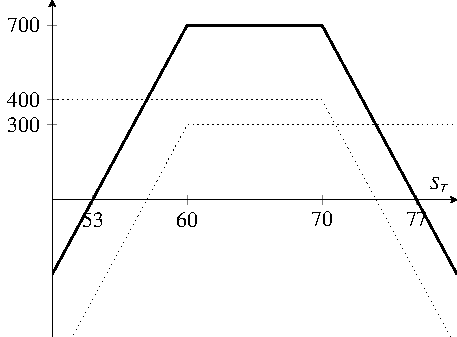
\includegraphics[width=0.8\textwidth]{IMG/fig20-3.pdf}
        \caption{卖出组合价差}
    \end{center}
\end{figure}

粗看上去,这似乎是一个比跨式价差更保守的策略,因为盈利范围更宽,股票需要运动相当大的幅度才会达到盈亏平衡点。在没有后续行动的情况下,这没有错。但是,如果股票一开始就迅速上涨或下跌,宽跨式价差卖出者常常没有其他选择,只能买回实值期权以限制他的亏损。正如前面所显示的,这时买回的价格有可能会包括大量的时间价值,从而产生显著的亏损。

宽跨式价差卖出者唯一可用的其他方法(除了通过交易把这个头寸平仓之外),是在股票达到任何一个盈亏平衡点时,将这个头寸转化为一手跨式价差。

如果前面示例里的 XYZ 价格上涨到了 70 或 71,1 月 70 看跌期权就会被卖掉。根据可用的质押金额,在卖掉 1 月 70 看跌期权的时候,可以买回也可以不买回 1 月 60 看跌期权。如果股票价格稳定下来,这种把宽跨式价差转化为跨式价差的做法就会效果很好。如果股票继续上涨,它也可以减少痛苦。不过,如果股票反转方向,1 月 70 看跌期权空头就无法盈利。在决定是否要将宽跨式价差转化为跨式价差上,标的股票的技术分析可以提供一定的帮助。如果股票价格有相当大的可能会回落,那也许就不值得将这手看跌期权向上挪仓。

在这个宽跨式价差的示例里,卖出者从卖出看跌期权和看涨期权中收入大笔的权利金。不过,\textbf{在许多时候,一个激进的宽跨式价差卖出者会想要卖出两手离到期日很近的虚值期权。}这些期权的卖价一般都不到 1 点。有的时候这是非常激进的策略,因为如果标的股票无论在哪个方向迅速运动,穿过行权价,这个卖出者就没有其他什么办法。他必须买回期权以限制亏损。不过,这类卖出宽跨式价差(卖出价格不到 1 点的短期虚值期权)对许多卖出者都有吸引力。\textcolor{red}{卖出价格不足 1 点的组合是一种拙劣的策略,应当避免这种策略。}
\section{对卖出未备兑跨式和宽跨式价差的进一步讨论}
我们在前面不断地提到,\textbf{看跌期权在变为实值期权后失去时间价值的速度要比看涨期权快}。交易者常常可以通过卖出 1 或 2 手额外的看跌期权来构建一个中性头寸。也就是说,如果交易者卖出 5 或 6 手看跌期权和 4 手条款相同的看涨期权,他常常可以创造出一个比跨式价差更为中性的头寸。如果股票向上运动,看涨期权在一个看多的市场里积累起时间价值,而额外的看跌期权则帮助抵消看涨期权的不利后果。另一方面,如果股票下跌,5 或 6 手看跌期权所拥有的时间价值和 4 手看涨期权一样多,这也是一个不带偏向的中性头寸。如果股票一开始就大幅下跌,卖出者总是可以通过卖出另外的 1 或 2 手看涨期权来保持平衡。卖出额外的 1 或 2 手看跌期权是跨式价差卖出者对付最凶险敌人的对策,这个敌人就是标的股票的迅速和极度上涨。